%Nach Subsubsection "Generierung der Skelettstruktur"
\subsubsection*{Skelett aus L-System generieren}
Ausgehend von einer Liste von Tupeln, die jeweils Start und Endpunkte einer von der Turtle gezeichneten Strecke enthalten wird das Skelett mit Unity Klassen generiert. Zunächst wird die Liste in eine Baumstruktur überführt. Dabei entspricht ein Knoten im Baum einem Knochen im Skelett. Zwei Knoten stehen in einer Eltern-Kind-Beziehung im Baum, wenn die zugehörigen Strecken sich schneiden. Dabei wird gefordert, dass der Endpunkt der zum Elternknoten gehörigen Strecke dem Startpunkt der zum Kindknoten gehörigen Strecke gleicht. Da angenommen wird, dass es zu jedem Startpunkt eines Tupels in der Liste ein weiteres Tupel gibt, dessen Endpunkt dem Startpunkt gleicht lässt sich der Baum so definieren. Der Baum wird traversiert und zu jedem Knoten wird ein GameObject erstellt.  Dieses wird mit einem Rigidbody, einem CapsuleCollider und einem primitiven Mesh versehen. Die Knochen werden in Kategorien, wie zum Beispiel Arm, Bein oder Kopf eingeteilt. Zwei Knochen werden mit einem Joint verbunden, wenn sie im Baum in einer Eltern-Kind-Beziehung stehen. Für die erlaubten Rotationen der Joints wurden Standardwerte je nach Kategorie festgelegt. Abbildung \ref{skeletonlsystemex} zeigt ein über ein L-System generiertes Skelett.

\begin{figure}[h]
\begin{center}
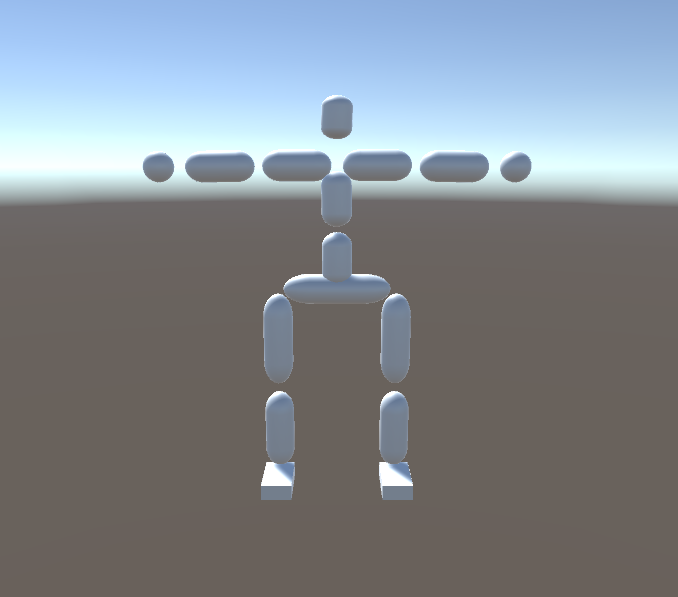
\includegraphics[width = 0.5\textwidth]{resources/img/skeletonlsystemex.png}
\end{center}
\caption{Mittels L-System generiertes Skelett}
\label{skeletonlsystemex}
\end{figure}